\newcommand{\suffix}[1]{$\text{suff}_{#1}$}

\chapter{Indexeren van vaste tekst}
\begin{itemize}
    \item Sommige zoekoperaties gebeuren op een vaste tekst $T$ waarin frequent gezocht wordt naar een veranderlijk patroon $P$.
    \item Voorbereidend werk op de tekst om efficiënter te doorzoeken.
    \item Alle zoekmethoden in hoofdstuk \ref{ch:zoeken_in_strings} verrichten voorbereidend werk op het patroon.
    \begin{itemize}
        \item In het slechtste geval is dit $O(t + p)$.
        \item Dit kan gereduceerd worden tot $O(p)$ door eerst $O(t)$ voorbereidend werk te doen op $T$.
        \item Via \textbf{suffixen}.
        \item Als een patroon in de tekst voorkomt, moet het een prefix zijn van één van de suffixen.
        \item Een suffix dat begint op lokatie $i$ wordt aangeduidt met \suffix{i}.
    \end{itemize}
\end{itemize}


\section{Suffixbomen}
\begin{figure}[ht]
    \centering
    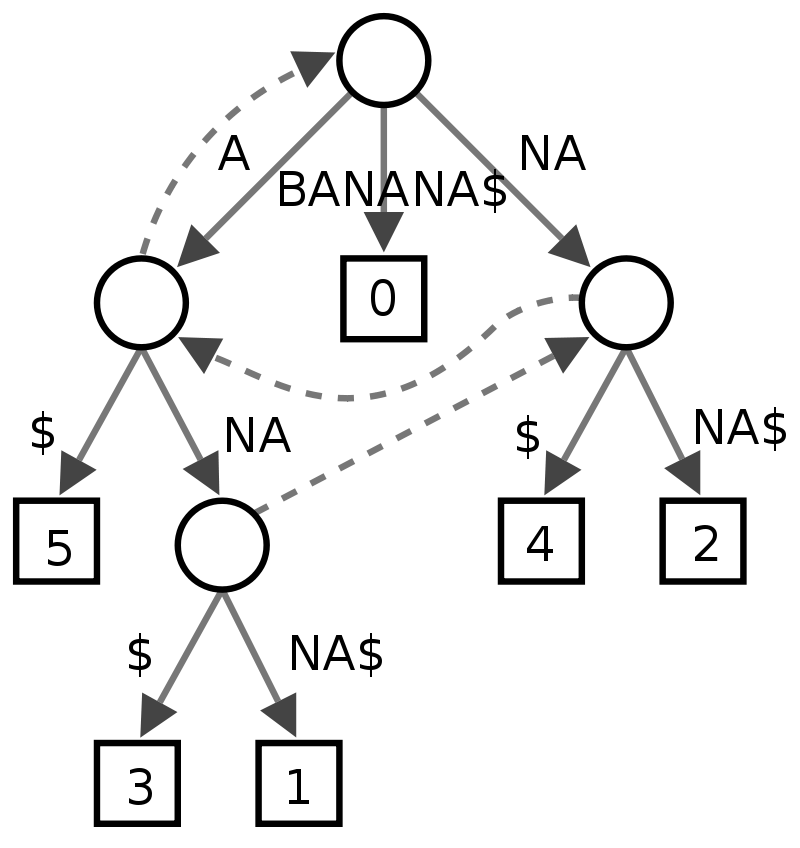
\includegraphics[width=0.5\textwidth]{suffix_tree}
    \caption{Een suffixboom voor het woord \texttt{BANANA\$}. Elk van de suffixen \texttt{BANANA\$}, \texttt{ANANA\$}, \texttt{NANA\$}, \texttt{ANA\$}, \texttt{NA\$} en \texttt{A\$} kan gevonden worden in deze boom. Het suffix \texttt{NANA\$} wordt gevonden door twee keer de rechterdeelboom te nemen vanuit de wortel. De index $2$ wijst erop dat de suffix begint bij $T[2]$. De gestreepte verbindingen zijn staartpointers.}
    \label{fig:suffix_tree}
\end{figure}
\begin{itemize}
    \item Gebaseerd op de  \textbf{Patriciatrie}.
    \item Het aantal inwendige knopen is $O(t)$ en de vereiste geheugenruimte is $O(|\Sigma|t)$.
    \item Kan geconstrueerd worden in $O(t)$.
    \item Er zijn een aantal \textbf{wijzigingen} ten opzichte van een originele Patriciatrie:
    \begin{enumerate}
        \item Een patriciatrie slaat strings op bij de bladeren. Hier volstaat de index $i$ van \suffix{i}.
        \item De testindex wordt vervangen door een begin- en eindindex, die een substring aangeeft van $T$ in elke knoop. 
        \item In elke inwendige knoop kan een staartpointer opgenomen worden.
        \begin{itemize}
            \item De \textbf{staart($s$)} van een string $s$ is de string bekomen door het eerste karakter te verwijderen.
            \item Er is een staartpointer van een inwendige knoop $x$ naar een andere inwendige knoop $y$ als de padstring van $y$ hetzelfde is als staart($s$).
            \item Op figuur \ref{fig:suffix_tree} is er bijvoorbeeld een staartpointer van de rechtse inwendige knoop met als padstring \texttt{NA} naar de linkse inwendige knoop met als padstring \texttt{A} omdat staart(\texttt{NA}) = \texttt{A}.
        \end{itemize}
    \end{enumerate}
    \item De voorwaarde dat een string geen prefix mag zijn van een ander werd vroeger opgelost door een extra afsluitend karakter te introduceren, maar dat is hier moeilijker.
    \begin{itemize}
        \item Elk karakter van $T$ wordt één per één toegevoegd in de suffixboom.
        \item Na $k$ iteraties zitten er suffixen van $T[0]\cdots T[k-1]$ in de boom zonder afsluitteken.


        \item \todo{...}
        \item Dus om ervoor te zorgen dat deze voorwaarde geldig is, moet $T$ eindigen op een karakter dat nergens anders voorkomt in de tekst. Op figuur \ref{fig:suffix_tree} is dit het karakter \texttt{\$}.
    \end{itemize}
\end{itemize}



\section{Suffixtabellen}
\begin{itemize}
    \item Eenvoudiger alternatief voor een suffixboom, maar vereist minder geheugen.
    \item Een tabel met de gerangschikte suffixen (hun startindices) van $T$.
    \alert Een suffixtabel bevat geen informatie over het gebruikte alfabet.
    \item Een suffixtabel construeren kan door eerst de suffixboom op te stellen in $O(t)$ en daarna deze in inorder te overlopen, ook in $O(t)$.
    \begin{itemize}
        \item De suffixtabel, geconstrueerd uit de suffixboom uit figuur \ref{fig:suffix_tree}.

    $$A = \begin{bmatrix}6 & 5 & 3 & 1 & 0 & 4 & 2\end{bmatrix}$$

        Het eerste element ($A[0] = 6$) is een verwijzing naar het eindkarakter, maar zit niet in de boom.
    \end{itemize}
    \item Er is echter nog een belangrijke hulpstructuur nodig, de LGP-tabel.
    \begin{itemize}
        \item Langste Gemeenschappelijke Prefix - tabel.
        \item Voor \suffix{i} is $LGP[i]$ de lengte van het langste gemeenschappelijke prefix van \suffix{i}.
        \item De alfabetische opvolger van \suffix{i} wordt gegeven door \textbf{opvolger(\suffix{SA_{|j|}}) = \suffix{SA_{|j + 1|}}}.
    \end{itemize}

    \item De LGP-tabel wordt opgesteld via de suffixtabel:
    \begin{itemize}
        \item Start met \suffix{0}.
        \item Zoek $j$ zodat $A[j] = 0$. 
        \item Bepaal het langste gemeenschappelijke suffix:
        \begin{itemize}
            \item Start met $l = 0$.
            \item Verhoog $l$ tot $T[i + l]$ niet meer overeenkomt.
        \end{itemize}
    \end{itemize}
    
\end{itemize}